\chapter{Power system protections}
\label{ch:protections}
\minitoc

Cause N-k (k = 2-5) contingencies

\cite{ProtectionMisoperationsBian2012}

\TODO{Pour chaque chapitre, passer plus de temps sur l'intro et la structure}


\TODO{When writing, think about the "topic sentence, example, analysis/development, point, link to next paragraph" structure. (Can be flexible)}

Modern numerical relays can self test, reducing hidden failure probability, but can still be misconfigured, and the circuit breaker can fail to open on demand.

Statistic frequency delayed clearing N-1?

\TODO{Protection indicator}
\section{Handling uncertain protection behaviour in simulations of cascading outages}

\section{Contingency selection}

\TODO{contingency types~\cite{ContingencyTypes}, future work: FMEA protection, missing vs unwanted trips., n-1-1 requires screening~\cite{VittalN-1-1}}

This chapter is partly based on the following publication:
\begin{itemize}
    \item \fullcite{ISGT2023_Protections}
\end{itemize}

As mentioned in the previous chapters, protections play a key role during cascading outages. Protections are usually designed to protect a given element against faults and abnormal conditions. The stability of the system as a whole plays a secondary (but still important) role in the design of protection systems. So, history has shown that even a protection operates ``as designed", it can sometimes contribute to the propagation of a cascade and sometimes prevent its propagation~\cite{PSRCreportProtectionMisop}. Another point to consider is that, as the system operates in a (potentially very) degraded state during cascading outages, protection misoperations (either unwanted or missing trips) can become likely and impact the propagation of the cascade.

Section~\ref{sec:protectionBasics} briefly reminds the basic protection principles. Then, section~\ref{sec:noteOnProtections} discusses the scope of considered protections in this thesis. Section~\ref{sec:protectionPerformance} reviews the most important (from a system reliability perspective) protection misoperations that can occur during/due to cascading outages. And section~\ref{sec:consideredProtections} concludes with a list of the protection models considered in this thesis.


\section{Power system protection basics}
\label{sec:protectionBasics}

% \begin{itemize}
    % \item (discrete fourier transform (DFT) but is not modelled in RMS tools)
    % \item Distance protection
    % \begin{itemize}
    %     \item Load encroachment
    % \end{itemize}
    % \item Differential
    % \item Overcurrent
    % \item UFLS/UVLS
    % \item etc.
% \end{itemize}

This section briefly introduces protections systems used in power systems. For a more complete overview, the reader is referred to textbooks on the subject. The book~\cite{HorowitzBook} has been used as a basis for this section.

\subsection{Components}

Protections systems usually consist of three main elements.

\begin{itemize}
    \item Transducers (i.e. voltage transformers (VTs) and current transformers (CTs)) that reduce the magnitude of electrical quantities to values that are easier to work with (e.g. voltages from 400~kV to 110~V and currents from 1000~A to 1~A.).
    \item A relay that measures those electrical quantities and applies some predetermined logics to decide when to trip.
    \item A circuit breaker (CB) that disconnects the protected element. Note that for elements connected to more than one terminal (e.g. lines), a protection system (including transducers, a relay and a circuit breaker) is placed at each terminal.
\end{itemize}

\subsection{Reliability, dependability and security}

The reliability of protection systems is decomposed into two concepts: dependability and security. Dependability is the measure of certainty that a protection will operate for all faults for which they are designed to operate (e.g. always trip when there is a fault on the protected line). Security (of a protection system, not to be confused with security of a power system) is the measure of certainty that a protection will not operate for faults other than the ones for which it is designed (e.g. never trip for faults on nearby lines). Most protection systems are designed for high-dependability. This is because allowing sustained (e.g. short-circuit) faults can cause important physical damage and even deaths. On the other hand, an isolated security issue (i.e. a protection incorrectly trips during normal operation) should have no consequences in a N-1 secure system. Security issues can however threaten the system stability when they occur following a fault or during a cascading outage. Balancing dependability and security is the most challenging aspect of protection system design.

\subsection{Most common line protection schemes}

The most common line protection schemes are reviewed below. Other types of elements (generators, transformers, etc.) can also use those schemes, but also other schemes. The latter are reviewed in the reference book.

\begin{itemize}
    \item Distance protection: the working principle of distance protections is shown in figure~\ref{fig:distanceFigure}. It is based on the fact that during a metallic short-circuit of a line, the ratio between the voltage and the current (called apparent impedance) measured by the relay is equal to the impedance of the portion of the line between the relay and the fault. If this measured impedance is smaller than the impedance of the entire line, it means that the fault is on the line and that the relay should open the line. In practice, uncertainties\footnote{Infeed from the other side of the fault, variation of line parameters due to variable sag, etc.} imply that the presence of a fault can only be guaranteed when the apparent impedance is lower than 80 to 90\% of the line impedance. Multiple ``zones" are thus necessary to protect a line. The most common zones definition is as follows: Zone 1 protects 80-90\% of the line and operates ``instantaneously" (i.e. with no intentional time delay). Zone 2 protects 110-120\% of the line (i.e. the full line with some margin) and operates with some time delay (e.g. 300~ms) to coordinate with the zone 1 of adjacent line(s). Together, zone 1 and zone 2 protect the full line. Using telecommunications, it is possible to have instantaneous operation for the full line. Additionally, a zone 3 is often used as a backup protection for the adjacent line(s). It thus covers the full line plus the longest adjacent line plus some margin. It operates with a larger time delay than zone 2 (e.g. 600~ms to 2~s). Distance protection is the main protection in transmission systems.
\begin{figure}
    \centering
    \includegraphics[width = 0.8\textwidth]{Figs/Distance.png}
    \caption{Basic schematic of distance protection~\cite{distanceFigure}}
    \label{fig:distanceFigure}
\end{figure}

    \item Differential protection: the working principle is that the sum of ingoing and outgoing currents in a given protected zone should be equal to zero according to Kirchhoff's law. A sum that is (significantly) different from zero indicates the presence of a fault and the necessity to trip. Due to the geographical expansions of line (dozens to hundreds of kilometres), it is necessary to have communication between both ends of a line to use differential protections. Differential protection is thus mostly used for extra high-voltage (EHV) lines (400~kV in Europe).

    \item Overcurrent protection: as the name indicates overcurrent protection disconnect the protected line when it is subject to high currents. It can either be definite-time (trips when the current is higher than a threshold for a given duration) or inverse-time (trips faster for more severe overcurrents). Overcurrent protection is only used as backup protection in transmission systems.
\end{itemize}

\subsection{Redundancy}

As for all critical systems, redundancy is used to increase the reliability of protection systems. This is especially true at higher voltage levels where higher levels of redundancy are used. The example in Figure~\ref{fig:protectionBackup} demonstrates the different kinds of backups used. In this example, there is a fault on line AB. The primary protection is the relay R\textsubscript{1} that sends a tripping signal to breaker B\textsubscript{1}. R\textsubscript{2} is the duplicate primary protection. It can be identical to R\textsubscript{1} or use a different scheme. The transducers and battery power supply can also be duplicated. The breaker is usually not duplicated due to its higher cost. R\textsubscript{3} is the local backup or breaker failure protection. If R\textsubscript{1} or R\textsubscript{2} sends a tripping signal but B\textsubscript{1} does not open, it will send a trip signal to B\textsubscript{6}, B\textsubscript{7} and B\textsubscript{8}. Breaker failure protection operates with a larger time delay than the primary protection. R\textsubscript{4}, R\textsubscript{9} and R\textsubscript{10} act as remote backup protection. Remote backup protection is often performed by zone 3 relays.

\begin{figure}
    \centering
    \includegraphics[width=0.8\linewidth]{Figs/ProtectionBackup.pdf}
    \caption{Duplicate primary, local backup, and remote backup protection~\cite{HorowitzBook}}
    \label{fig:protectionBackup}
\end{figure}

\textbf{Note:} in its final version, this thesis will include a paragraph on substation configurations, the generic configuration(s) used in the test systems and statistical data on failure rates. More information on substation configurations can be found in~\cite{3rdZoneRevisited}

% Busbar arrangement, breaker failure protection (Ciapessoni presentation, typical scheme to balance the busbar)

% \begin{figure}
%     \centering
%     \includegraphics[width=0.6\linewidth]{Figs/Busbar.pdf}
%     \caption{Typical substation bus arrangements: (a) single bus, single breaker; (b) two buses, one breaker; (c) two buses, two breakers; (d) ring bus; and (e) breaker-and-a-half~\cite{HorowitzBook}}
%     \label{fig:my_label}
% \end{figure}


\section{Note on the protection models used in this thesis}
\label{sec:noteOnProtections}

The main objective of this thesis is to design a methodology for probabilistic dynamic security assessment of power systems. While probabilistic dynamic security assessment could be useful to help protection design, it is not the main objective as a satisfactory security assessment methodology has to be designed first. The protection models used in this thesis were thus chosen to satisfy two criteria. The models should lead to a relatively accurate estimation of the risk\footnote{It should be noted that, even if using more complex models, the exact value of the risk (in MWh/y or €/y) is of low significance. What is important is to be able to compare the risk associated with different scenarios and to be able to identify actions that most effectively reduce the risk.} and realistic cascading outage scenarios\footnote{The IEEE CFWG also recommends verifying that the methodology leads to cascading outage sizes that follow a power law~\cite{Benchmarking2016}. The validation of the methodology is discussed in more details in chapter~\ref{ch:DPSA}.} such that (i) the added value of the method compared to QSS methodologies can be shown, (ii) variance reduction techniques used in the probabilistic methodology have similar performance than with more elaborated models. To explain the second criteria, it is necessary to briefly introduce probabilistic methods. Probabilistic methods often use Monte Carlo (MC) methods to handle uncertainties. The issue with basic MC is that, as power system are very reliable, most MC simulations lead to scenarios with no consequences which waste computational resources. Techniques that increase the likelihood of sampling more ``interesting" scenarios (i.e. scenarios that contribute more to the total risk) are thus necessary. Those techniques can loosely be referred to as variance reduction techniques. The two criteria are quite abstract, but the main idea is to focus on protections that have the highest impact on the risk. This can be done through study of past cascading outages and experience.

It is difficult to obtain data regarding the exact protection design used by TSOs. Also, this data does not exist for academic test systems. It is thus necessary to use generic protection settings. If a TSO applies the methodology, they should have access to a database of protection settings. On the other hand, they initially might not have all protection models in their dynamic simulator, nor the interface necessary to automatically bring the protection settings to the simulator. They will thus likely also use the methodology with generic protection models. The methodology will then show what settings to modify to reduce the risk of cascading outages. It can then be a good exercise to compare those settings (obtained in a greenfield environment with a focus on system security) and the ones designed by protection engineers (in brownfield, with a focus on dependability, and with additional concerns regarding resistive faults, different types of fault, etc.).


\section{Protection performance during system disturbances}
\label{sec:protectionPerformance}

As power system are drawn far from normal operation during cascading outages, protections are more likely to misoperate. Possible misoperations have been reported by the IEEE Power System Relaying and Control Committee (PSRC) in a report~\cite{PSRCreportProtectionMisop}, its summary~\cite{PSRCreportSummaryProtectionMisop} and in previous works~\cite{ProtectionFailuresDemetrios}. However, as mentioned above, only the misoperations that contributed most to the risk in previous blackouts are considered. The misoperations considered are more similar to the smaller list of misoperations given in~\cite[ch3]{ENTSOEdefencePlan} (that is itself based on~\cite{PSRCreportProtectionMisop, PSRCreportSummaryProtectionMisop, ProtectionFailuresDemetrios}).

On top of those misoperations that are linked with the system degraded state, the possibility of a relay not operating simply because the relay (or its transducers, power supply or CB) is failed has to be considered.

% Issues in~\cite{PSRCreportProtectionMisop} that can be solved with modern numerical relays, legacy issues of electromech and solid-state are not considered. On the other hand, but only relays based on phasor\footnote{Could be implicit, reduce inverter current capacity to account for negative sequence injection.}.

\textbf{Note:} the final thesis will include more details on the misoperations that are not considered and the reasons for not considering them.

\subsection{Distance protection}

Distance protection misoperations are the most common type of misoperations. Zone 3 is the one that causes the most issues. This is because zone 3 has to overreach in order to provide backup for adjacent lines. During large disturbances, this zone is thus susceptible to trip even in the absence of fault. The three main causes for unwanted operations of zone 3 relays are listed below.

\begin{itemize}
    \item High demand: higher line currents imply that the apparent impedance measured by relays decreases (if voltage is roughly constant). In some extreme cases, this can cause the apparent impedance to enter zone 3 or even zone 2. To avoid this issue, a load blinder must be used as shown in Figure~\ref{fig:encroachment}. According to NERC's (North American Electric Reliability Council) requirements, the distance protection must not trip for currents 1.5 times the maximum current line rating (considering dynamic line rating) at 85\% of nominal voltage and for a power factor of 30 degrees~\cite{PSRCreportProtectionMisop}. Such a load blinder is thus used in our model.
\begin{figure}
    \centering
    \includegraphics[width=0.8\linewidth]{Figs/LoadEncroachment.jpg}
    \caption{Load encroachment. The green zones are quadrilateral zones used by modern numerical relays. The red zones are mho characteristics mostly used by old electromechanical relays~\cite{LoadEncroachmentFig}}
    \label{fig:encroachment}
\end{figure}
    \item Power swings: large (potentially stable) power swings can cause distance relay to misoperate. To illustrate this, consider the following example. A test system consists of two synchronous generators connected by a single line. During a stable system swing, the angle difference between the two generators can be up to 180 degrees\footnote{According to the basic equal area criterion model.}. The voltage at the electrical centre of the network (here the middle of the line) is then 0 (sum of the voltages of the two generators assuming the magnitudes of the voltages are equal). From the relay point of view, this is equivalent to a metallic three-phase fault. The difference is that power swings develop on longer time scales than short-circuits. Relays can thus use a power swing blocking (PSB) function to distinguish between faults and swings. The model of PSB used in this thesis is still to be defined.
    \item Voltage instability: during voltage collapses, voltages decrease and loads tend to draw more current to partially maintain a constant power. For relays, this causes a reduction of the apparent impedance and potentially trips in zone 3 or zone 2. Similarly to power swing, the difference compared to actual fault is that voltage instabilities develop slower. However, there is no standard method to distinguish between voltage instabilities and power swings. PSB can thus be used for both. As PSBs typically reset after 2~s, the voltage collapse should be stopped faster to avoid tripping of distance relays. It should be noted that while tripping due to a voltage instability is usually unwanted, it can in some case limit the propagation of the cascade by isolating the zone where the voltage instability takes place.
\end{itemize}

Some other types of misoperations are given in~\cite{PSRCreportProtectionMisop} but not considered in this thesis. For example, currently installed numerical relays use methods like discrete Fourier transform (DFT) to evaluate phasor quantities (voltage and currents) used in the protection logics. This introduces inaccuracies during frequency deviations. However, those inaccuracies are relatively minor (up to 10\% during very large frequency deviations) and affect all relays in the same way as the frequency is usually uniform in the whole system (or in a given island is the system is split). Those inaccuracies thus cannot significantly change the order of operations of protections. It is thus expected that neglecting this effect should not have a high impact on the possible cascading scenarios nor on their consequences.

Distance protection of multiterminal lines (lines with three or more connections) requires additional considerations. However, as academic test systems do not include such lines, those issues are not considered here.

% For distance relay quadrilateral characteristic, the use of memory voltage is not as prone to cause misoperations during frequency excursions as for the mho elements. The reason for this is that the memory voltage is used for directional measurement only, and not for reach. It is possible that a large frequency variation could cause loss-of-directionality of the quadrilateral characteristic, but undesired tripping would still not occur as the apparent impedance would be outside the set reactive and resistive reach. However it could result in a missed trip for a forward fault or a trip for a reverse fault if the directional element makes an erroneous decision.

\subsection{Overcurrent protection}

Line overcurrent protection is only ever used as a backup protection. It is thus expected to have little impact during cascading outages~\cite{PSRCreportProtectionMisop}. Ref.~\cite{PSRCreportProtectionMisop} mentions possible misoperation of the ground overcurrent element for untransposed lines (those lines are unbalanced and thus generate zero (and negative) sequence currents even when only positive sequence voltages are present). With numerical relays, it is however possible to solve this issue by restraining the ground element by a fraction (e.g. 10\%) of the positive sequence current. This issue is thus not considered.

Overcurrent protection is sometimes installed on transformers to backup the differential protection and to protect the transformer against overcurrents (that reduce its lifetime). Typical settings for overcurrent protection of transformers is to trip for 130-200\% of the transformer rating~\cite{ENTSOEdefencePlan}.

\subsection{Differential protection}

Due to its design, differential protection is mostly insensitive to system disturbances. The main reasons it is not the only type of protection used are the need for a communication medium (in the case of lines) and inability to act as a backup for elements outside of the protected zone. Some possible misoperations are given in~\cite{PSRCreportProtectionMisop} but are not considered here.


% Busbar protection very reliable so does not misoperate, can consider busbar fault as an initiating event (less likely than line fault).

\section{Summary of protection models used}
\label{sec:consideredProtections}

The generic protection models used in this thesis are listed below. These models include the considerations given in section~\ref{sec:protectionPerformance} as well as relatively standard protection models used in other (probabilistic or even deterministic) dynamic security assessment studies. Note that, by default, all protections that are said to operate instantaneously (or with no intentional time delay) are supposed to operate in 100~ms (this corresponds roughly to 20~ms for the relay to take the decision and 80~ms for the CB opening)\footnote{The probability distribution of this time must still be defined}.

\subsection{Line protection}

Lines are supposed to be protected by a distance and a differential relay. Actually, since no misoperations of differential relays are considered, differential relays are not explicitly modelled in the power system simulator. The differential protection only implies that faults will be cleared instantaneously for the whole line, not only the part that is covered by zone 1. Also, it reduces the likelihood of missing trip (discussed in more details in the final thesis, pilot distance protection will also be discussed).

Zone 1 protects 80\% of the line and operates instantaneously. Zone 2 protects 120\% of the line and operates with a 300~ms delay (including CB opening time\footnote{To be confirmed.}). Zone 3 setting is more complex due to infeed effects. It still has to be defined. Load encroachment of 150\% of the maximum line current at 85\% of the voltage with a 30 degrees power factor is also included. Finally, a PSB function is also added (exact model to be defined).

Since only three-phase faults are considered (due to the use of a RMS (root mean square) simulator), auto-reclosing of lines is not considered.


\subsection{Generator protection}

Generators must be protected against undervoltage (that cause degraded performance of auxiliaries), over- and underfrequency, overexcitation and out-of-step conditions. Thus the following protections are used:

\begin{itemize}
    \item Undervoltage protection: this is especially critical for nuclear generators. For those an instantaneous undervoltage protection set at 0.9~pu is used. For other types of generators, a less strict protection can be used. \TODO{\url{https://eepublicdownloads.entsoe.eu/clean-documents/pre2015/consultations/Network_Code_RfG/120626_-_NC_RfG_-_Requirements_in_the_context_of_present_practices.pdf} says requirement for all is 0.9 forever, 0.85 for 60ms (a bit country dependent).}
    \item Under- and overfrequency: past blackouts (e.g. the 2003 Italy blackout) have shown that distributed generators tend to unexpectedly disconnect during frequency excursions. In this thesis, it is assumed that generators connected on the transmission side strictly follow ENTSO-E requirements for continental Europe~\cite{ENTSOEgeneratorRequirements}. So, instantaneous protection is used for frequencies outside of the range 47.5-51.5~Hz. According to~\cite{PSRCreportProtectionMisop}, hydro units can operate in a large band of frequency. Generators connected to the distribution side are discussed in more details in chapter~\ref{ch:distrib}.
    \item Overexcitation: Volt-per-Hertz protection is used. The settings are still to be defined.
    \item Out-of-step: a simple model of out-of-step protection is used. The generator trips instantaneously when the angle difference between the generator and the centre of mass of the system (or the island if the system is split) is larger than 180 degrees.
\end{itemize}

Under- and overexcitations limiters are also considered although they are not stricto sensu protections.


\subsection{System protection}

Undervoltage load shedding (UVLS) is not used by all TSOs and is thus not considered in this thesis. Underfrequency load shedding (UFLS) is used following ENTSO-E standards~\cite{ENTSOE-UFLS}. More precisely, UFLS instantaneously disconnects load by steps between 49 and 48~Hz. The number and size of steps are still to be defined.

Special protection schemes (SPSs) can also be considered. However, since they are designed to mitigate a specific weakness of a given system, it is not possible to define a generic model of a SPS. SPSs are discussed in chapter~\ref{ch:SPS}.

\subsection{Transformer protection}

An instantaneous overcurrent protection set at 150\% of the rating of the transformer is used. No inverse-time protection is used. To be confirmed.

\subsection{Protections on the distribution side}

This is discussed in more details in chapter~\ref{ch:distrib}. Generator and motor protections are considered, but not line protections.
